\documentclass[twoside]{book}

% Packages required by doxygen
\usepackage{fixltx2e}
\usepackage{calc}
\usepackage{doxygen}
\usepackage[export]{adjustbox} % also loads graphicx
\usepackage{graphicx}
\usepackage[utf8]{inputenc}
\usepackage{makeidx}
\usepackage{multicol}
\usepackage{multirow}
\PassOptionsToPackage{warn}{textcomp}
\usepackage{textcomp}
\usepackage[nointegrals]{wasysym}
\usepackage[table]{xcolor}

% Font selection
\usepackage[T1]{fontenc}
\usepackage[scaled=.90]{helvet}
\usepackage{courier}
\usepackage{amssymb}
\usepackage{sectsty}
\renewcommand{\familydefault}{\sfdefault}
\allsectionsfont{%
  \fontseries{bc}\selectfont%
  \color{darkgray}%
}
\renewcommand{\DoxyLabelFont}{%
  \fontseries{bc}\selectfont%
  \color{darkgray}%
}
\newcommand{\+}{\discretionary{\mbox{\scriptsize$\hookleftarrow$}}{}{}}

% Page & text layout
\usepackage{geometry}
\geometry{%
  a4paper,%
  top=2.5cm,%
  bottom=2.5cm,%
  left=2.5cm,%
  right=2.5cm%
}
\tolerance=750
\hfuzz=15pt
\hbadness=750
\setlength{\emergencystretch}{15pt}
\setlength{\parindent}{0cm}
\setlength{\parskip}{0.2cm}
\makeatletter
\renewcommand{\paragraph}{%
  \@startsection{paragraph}{4}{0ex}{-1.0ex}{1.0ex}{%
    \normalfont\normalsize\bfseries\SS@parafont%
  }%
}
\renewcommand{\subparagraph}{%
  \@startsection{subparagraph}{5}{0ex}{-1.0ex}{1.0ex}{%
    \normalfont\normalsize\bfseries\SS@subparafont%
  }%
}
\makeatother

% Headers & footers
\usepackage{fancyhdr}
\pagestyle{fancyplain}
\fancyhead[LE]{\fancyplain{}{\bfseries\thepage}}
\fancyhead[CE]{\fancyplain{}{}}
\fancyhead[RE]{\fancyplain{}{\bfseries\leftmark}}
\fancyhead[LO]{\fancyplain{}{\bfseries\rightmark}}
\fancyhead[CO]{\fancyplain{}{}}
\fancyhead[RO]{\fancyplain{}{\bfseries\thepage}}
\fancyfoot[LE]{\fancyplain{}{}}
\fancyfoot[CE]{\fancyplain{}{}}
\fancyfoot[RE]{\fancyplain{}{\bfseries\scriptsize Generated on Tue May 10 2016 17\+:33\+:33 for Test\+Web\+Project by Doxygen }}
\fancyfoot[LO]{\fancyplain{}{\bfseries\scriptsize Generated on Tue May 10 2016 17\+:33\+:33 for Test\+Web\+Project by Doxygen }}
\fancyfoot[CO]{\fancyplain{}{}}
\fancyfoot[RO]{\fancyplain{}{}}
\renewcommand{\footrulewidth}{0.4pt}
\renewcommand{\chaptermark}[1]{%
  \markboth{#1}{}%
}
\renewcommand{\sectionmark}[1]{%
  \markright{\thesection\ #1}%
}

% Indices & bibliography
\usepackage{natbib}
\usepackage[titles]{tocloft}
\setcounter{tocdepth}{3}
\setcounter{secnumdepth}{5}
\makeindex

% Hyperlinks (required, but should be loaded last)
\usepackage{ifpdf}
\ifpdf
  \usepackage[pdftex,pagebackref=true]{hyperref}
\else
  \usepackage[ps2pdf,pagebackref=true]{hyperref}
\fi
\hypersetup{%
  colorlinks=true,%
  linkcolor=blue,%
  citecolor=blue,%
  unicode%
}

% Custom commands
\newcommand{\clearemptydoublepage}{%
  \newpage{\pagestyle{empty}\cleardoublepage}%
}


%===== C O N T E N T S =====

\begin{document}

% Titlepage & ToC
\hypersetup{pageanchor=false,
             bookmarks=true,
             bookmarksnumbered=true,
             pdfencoding=unicode
            }
\pagenumbering{roman}
\begin{titlepage}
\vspace*{7cm}
\begin{center}%
{\Large Test\+Web\+Project \\[1ex]\large bounswegroup5 }\\
\vspace*{1cm}
{\large Generated by Doxygen 1.8.10}\\
\vspace*{0.5cm}
{\small Tue May 10 2016 17:33:33}\\
\end{center}
\end{titlepage}
\clearemptydoublepage
\tableofcontents
\clearemptydoublepage
\pagenumbering{arabic}
\hypersetup{pageanchor=true}

%--- Begin generated contents ---
\chapter{Namespace Index}
\section{Packages}
Here are the packages with brief descriptions (if available)\+:\begin{DoxyCompactList}
\item\contentsline{section}{\hyperlink{namespacecom}{com} }{\pageref{namespacecom}}{}
\item\contentsline{section}{\hyperlink{namespacecom_1_1example}{com.\+example} }{\pageref{namespacecom_1_1example}}{}
\item\contentsline{section}{\hyperlink{namespacecom_1_1example_1_1servlets}{com.\+example.\+servlets} }{\pageref{namespacecom_1_1example_1_1servlets}}{}
\end{DoxyCompactList}

\chapter{Hierarchical Index}
\section{Class Hierarchy}
This inheritance list is sorted roughly, but not completely, alphabetically\+:\begin{DoxyCompactList}
\item \contentsline{section}{com.\+example.\+servlets.\+Atakan\+Servlet.\+Mathematician}{\pageref{classcom_1_1example_1_1servlets_1_1_atakan_servlet_1_1_mathematician}}{}
\item Http\+Servlet\begin{DoxyCompactList}
\item \contentsline{section}{com.\+example.\+servlets.\+Atakan\+Servlet}{\pageref{classcom_1_1example_1_1servlets_1_1_atakan_servlet}}{}
\item \contentsline{section}{com.\+example.\+servlets.\+Bugra\+Servlet}{\pageref{classcom_1_1example_1_1servlets_1_1_bugra_servlet}}{}
\item \contentsline{section}{com.\+example.\+servlets.\+Burak\+Servlet}{\pageref{classcom_1_1example_1_1servlets_1_1_burak_servlet}}{}
\item \contentsline{section}{com.\+example.\+servlets.\+Hello\+Servlet}{\pageref{classcom_1_1example_1_1servlets_1_1_hello_servlet}}{}
\item \contentsline{section}{com.\+example.\+servlets.\+Kerim\+Servlet}{\pageref{classcom_1_1example_1_1servlets_1_1_kerim_servlet}}{}
\item \contentsline{section}{com.\+example.\+servlets.\+Ozer2\+Servlet}{\pageref{classcom_1_1example_1_1servlets_1_1_ozer2_servlet}}{}
\item \contentsline{section}{com.\+example.\+servlets.\+Umut\+Servlet}{\pageref{classcom_1_1example_1_1servlets_1_1_umut_servlet}}{}
\item \contentsline{section}{Sevda\+Servlet}{\pageref{class_sevda_servlet}}{}
\end{DoxyCompactList}
\end{DoxyCompactList}

\chapter{Class Index}
\section{Class List}
Here are the classes, structs, unions and interfaces with brief descriptions\+:\begin{DoxyCompactList}
\item\contentsline{section}{\hyperlink{classcom_1_1example_1_1servlets_1_1_atakan_servlet}{com.\+example.\+servlets.\+Atakan\+Servlet} }{\pageref{classcom_1_1example_1_1servlets_1_1_atakan_servlet}}{}
\item\contentsline{section}{\hyperlink{classcom_1_1example_1_1servlets_1_1_bugra_servlet}{com.\+example.\+servlets.\+Bugra\+Servlet} }{\pageref{classcom_1_1example_1_1servlets_1_1_bugra_servlet}}{}
\item\contentsline{section}{\hyperlink{classcom_1_1example_1_1servlets_1_1_burak_servlet}{com.\+example.\+servlets.\+Burak\+Servlet} }{\pageref{classcom_1_1example_1_1servlets_1_1_burak_servlet}}{}
\item\contentsline{section}{\hyperlink{classcom_1_1example_1_1servlets_1_1_hello_servlet}{com.\+example.\+servlets.\+Hello\+Servlet} }{\pageref{classcom_1_1example_1_1servlets_1_1_hello_servlet}}{}
\item\contentsline{section}{\hyperlink{classcom_1_1example_1_1servlets_1_1_kerim_servlet}{com.\+example.\+servlets.\+Kerim\+Servlet} \\*This class is written for the personal assignment 6 }{\pageref{classcom_1_1example_1_1servlets_1_1_kerim_servlet}}{}
\item\contentsline{section}{\hyperlink{classcom_1_1example_1_1servlets_1_1_ozer2_servlet}{com.\+example.\+servlets.\+Ozer2\+Servlet} }{\pageref{classcom_1_1example_1_1servlets_1_1_ozer2_servlet}}{}
\item\contentsline{section}{\hyperlink{class_sevda_servlet}{Sevda\+Servlet} }{\pageref{class_sevda_servlet}}{}
\item\contentsline{section}{\hyperlink{classcom_1_1example_1_1servlets_1_1_umut_servlet}{com.\+example.\+servlets.\+Umut\+Servlet} }{\pageref{classcom_1_1example_1_1servlets_1_1_umut_servlet}}{}
\end{DoxyCompactList}

\chapter{File Index}
\section{File List}
Here is a list of all files with brief descriptions\+:\begin{DoxyCompactList}
\item\contentsline{section}{src/com/example/servlets/\hyperlink{_atakan_servlet_8java}{Atakan\+Servlet.\+java} }{\pageref{_atakan_servlet_8java}}{}
\item\contentsline{section}{src/com/example/servlets/\hyperlink{_bugra_servlet_8java}{Bugra\+Servlet.\+java} }{\pageref{_bugra_servlet_8java}}{}
\item\contentsline{section}{src/com/example/servlets/\hyperlink{_burak_servlet_8java}{Burak\+Servlet.\+java} }{\pageref{_burak_servlet_8java}}{}
\item\contentsline{section}{src/com/example/servlets/\hyperlink{_hello_servlet_8java}{Hello\+Servlet.\+java} }{\pageref{_hello_servlet_8java}}{}
\item\contentsline{section}{src/com/example/servlets/\hyperlink{_kerim_servlet_8java}{Kerim\+Servlet.\+java} }{\pageref{_kerim_servlet_8java}}{}
\item\contentsline{section}{src/com/example/servlets/\hyperlink{_ozer2_servlet_8java}{Ozer2\+Servlet.\+java} }{\pageref{_ozer2_servlet_8java}}{}
\item\contentsline{section}{src/com/example/servlets/\hyperlink{_sevda_servlet_8java}{Sevda\+Servlet.\+java} }{\pageref{_sevda_servlet_8java}}{}
\item\contentsline{section}{src/com/example/servlets/\hyperlink{_umut_servlet_8java}{Umut\+Servlet.\+java} }{\pageref{_umut_servlet_8java}}{}
\end{DoxyCompactList}

\chapter{Namespace Documentation}
\hypertarget{namespacecom}{}\section{Package com}
\label{namespacecom}\index{com@{com}}
\subsection*{Packages}
\begin{DoxyCompactItemize}
\item 
package \hyperlink{namespacecom_1_1example}{example}
\end{DoxyCompactItemize}

\hypertarget{namespacecom_1_1example}{}\section{Package com.\+example}
\label{namespacecom_1_1example}\index{com.\+example@{com.\+example}}
\subsection*{Packages}
\begin{DoxyCompactItemize}
\item 
package \hyperlink{namespacecom_1_1example_1_1servlets}{servlets}
\end{DoxyCompactItemize}

\hypertarget{namespacecom_1_1example_1_1servlets}{}\section{Package com.\+example.\+servlets}
\label{namespacecom_1_1example_1_1servlets}\index{com.\+example.\+servlets@{com.\+example.\+servlets}}
\subsection*{Classes}
\begin{DoxyCompactItemize}
\item 
class \hyperlink{classcom_1_1example_1_1servlets_1_1_atakan_servlet}{Atakan\+Servlet}
\item 
class \hyperlink{classcom_1_1example_1_1servlets_1_1_bugra_servlet}{Bugra\+Servlet}
\item 
class \hyperlink{classcom_1_1example_1_1servlets_1_1_burak_servlet}{Burak\+Servlet}
\item 
class \hyperlink{classcom_1_1example_1_1servlets_1_1_hello_servlet}{Hello\+Servlet}
\item 
class \hyperlink{classcom_1_1example_1_1servlets_1_1_kerim_servlet}{Kerim\+Servlet}
\begin{DoxyCompactList}\small\item\em This class is written for the personal assignment 6. \end{DoxyCompactList}\item 
class \hyperlink{classcom_1_1example_1_1servlets_1_1_ozer2_servlet}{Ozer2\+Servlet}
\item 
class \hyperlink{classcom_1_1example_1_1servlets_1_1_umut_servlet}{Umut\+Servlet}
\end{DoxyCompactItemize}

\chapter{Class Documentation}
\hypertarget{classcom_1_1example_1_1servlets_1_1_atakan_servlet}{}\section{com.\+example.\+servlets.\+Atakan\+Servlet Class Reference}
\label{classcom_1_1example_1_1servlets_1_1_atakan_servlet}\index{com.\+example.\+servlets.\+Atakan\+Servlet@{com.\+example.\+servlets.\+Atakan\+Servlet}}
Inheritance diagram for com.\+example.\+servlets.\+Atakan\+Servlet\+:\begin{figure}[H]
\begin{center}
\leavevmode
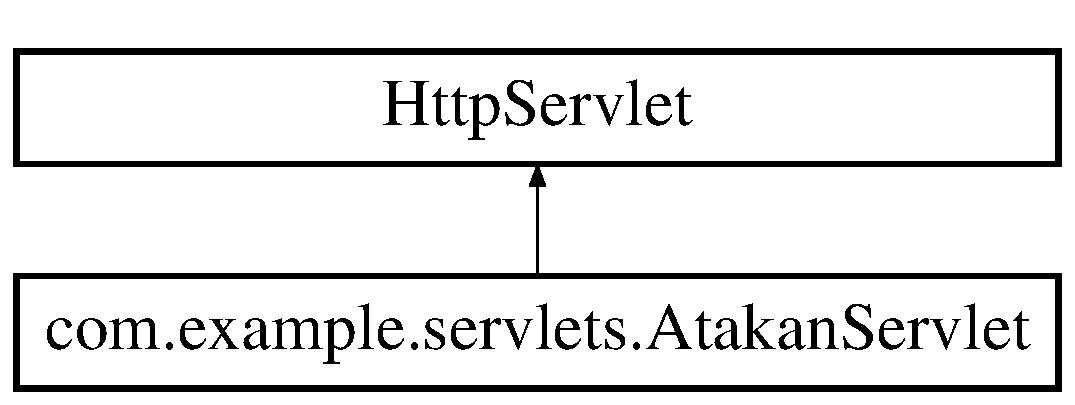
\includegraphics[height=2.000000cm]{classcom_1_1example_1_1servlets_1_1_atakan_servlet}
\end{center}
\end{figure}
\subsection*{Public Member Functions}
\begin{DoxyCompactItemize}
\item 
\hyperlink{classcom_1_1example_1_1servlets_1_1_atakan_servlet_a87e2532962ccd888df5a6e642ab6c047}{Atakan\+Servlet} ()
\item 
void \hyperlink{classcom_1_1example_1_1servlets_1_1_atakan_servlet_a6e8d25b648ac5982a2841efc984554f0}{drop\+Save\+Table} ()
\item 
void \hyperlink{classcom_1_1example_1_1servlets_1_1_atakan_servlet_a35d1a337e700fae93e6c1bc1e8caa3be}{create\+Save\+Table} ()
\item 
void \hyperlink{classcom_1_1example_1_1servlets_1_1_atakan_servlet_a58d74748199c3d7e4c4fc4a4dc4a4a9e}{create\+Table} ()
\item 
void \hyperlink{classcom_1_1example_1_1servlets_1_1_atakan_servlet_a8d4a40b18eb4548d16c072701c7eae16}{drop\+Table} ()
\item 
void \hyperlink{classcom_1_1example_1_1servlets_1_1_atakan_servlet_a12f494a4d42fef16831bba384424cba5}{search} (String search\+Query, Print\+Writer out)
\item 
void \hyperlink{classcom_1_1example_1_1servlets_1_1_atakan_servlet_ac43c5246ad7474fb542684e70b884f14}{create\+Database} ()
\end{DoxyCompactItemize}
\subsection*{Protected Member Functions}
\begin{DoxyCompactItemize}
\item 
void \hyperlink{classcom_1_1example_1_1servlets_1_1_atakan_servlet_a958df833cc34bf6033b56121d82459d1}{do\+Get} (Http\+Servlet\+Request request, Http\+Servlet\+Response response)  throws Servlet\+Exception, I\+O\+Exception 
\item 
void \hyperlink{classcom_1_1example_1_1servlets_1_1_atakan_servlet_ac40ca8b0badf1b9e4ef13f6ba72bf3b6}{do\+Post} (Http\+Servlet\+Request request, Http\+Servlet\+Response response)  throws Servlet\+Exception, I\+O\+Exception 
\end{DoxyCompactItemize}
\subsection*{Static Private Attributes}
\begin{DoxyCompactItemize}
\item 
static final long \hyperlink{classcom_1_1example_1_1servlets_1_1_atakan_servlet_a11981eeac794fddff011e967e18e28fb}{serial\+Version\+U\+ID} = 1L
\end{DoxyCompactItemize}


\subsection{Detailed Description}
Servlet implementation class \hyperlink{classcom_1_1example_1_1servlets_1_1_atakan_servlet}{Atakan\+Servlet} 

\subsection{Constructor \& Destructor Documentation}
\index{com\+::example\+::servlets\+::\+Atakan\+Servlet@{com\+::example\+::servlets\+::\+Atakan\+Servlet}!Atakan\+Servlet@{Atakan\+Servlet}}
\index{Atakan\+Servlet@{Atakan\+Servlet}!com\+::example\+::servlets\+::\+Atakan\+Servlet@{com\+::example\+::servlets\+::\+Atakan\+Servlet}}
\subsubsection[{\texorpdfstring{Atakan\+Servlet()}{AtakanServlet()}}]{\setlength{\rightskip}{0pt plus 5cm}com.\+example.\+servlets.\+Atakan\+Servlet.\+Atakan\+Servlet (
\begin{DoxyParamCaption}
{}
\end{DoxyParamCaption}
)}\hypertarget{classcom_1_1example_1_1servlets_1_1_atakan_servlet_a87e2532962ccd888df5a6e642ab6c047}{}\label{classcom_1_1example_1_1servlets_1_1_atakan_servlet_a87e2532962ccd888df5a6e642ab6c047}
\begin{DoxySeeAlso}{See also}
Http\+Servlet\+::\+Http\+Servlet() 
\end{DoxySeeAlso}


\subsection{Member Function Documentation}
\index{com\+::example\+::servlets\+::\+Atakan\+Servlet@{com\+::example\+::servlets\+::\+Atakan\+Servlet}!create\+Database@{create\+Database}}
\index{create\+Database@{create\+Database}!com\+::example\+::servlets\+::\+Atakan\+Servlet@{com\+::example\+::servlets\+::\+Atakan\+Servlet}}
\subsubsection[{\texorpdfstring{create\+Database()}{createDatabase()}}]{\setlength{\rightskip}{0pt plus 5cm}void com.\+example.\+servlets.\+Atakan\+Servlet.\+create\+Database (
\begin{DoxyParamCaption}
{}
\end{DoxyParamCaption}
)}\hypertarget{classcom_1_1example_1_1servlets_1_1_atakan_servlet_ac43c5246ad7474fb542684e70b884f14}{}\label{classcom_1_1example_1_1servlets_1_1_atakan_servlet_ac43c5246ad7474fb542684e70b884f14}
\index{com\+::example\+::servlets\+::\+Atakan\+Servlet@{com\+::example\+::servlets\+::\+Atakan\+Servlet}!create\+Save\+Table@{create\+Save\+Table}}
\index{create\+Save\+Table@{create\+Save\+Table}!com\+::example\+::servlets\+::\+Atakan\+Servlet@{com\+::example\+::servlets\+::\+Atakan\+Servlet}}
\subsubsection[{\texorpdfstring{create\+Save\+Table()}{createSaveTable()}}]{\setlength{\rightskip}{0pt plus 5cm}void com.\+example.\+servlets.\+Atakan\+Servlet.\+create\+Save\+Table (
\begin{DoxyParamCaption}
{}
\end{DoxyParamCaption}
)}\hypertarget{classcom_1_1example_1_1servlets_1_1_atakan_servlet_a35d1a337e700fae93e6c1bc1e8caa3be}{}\label{classcom_1_1example_1_1servlets_1_1_atakan_servlet_a35d1a337e700fae93e6c1bc1e8caa3be}
\index{com\+::example\+::servlets\+::\+Atakan\+Servlet@{com\+::example\+::servlets\+::\+Atakan\+Servlet}!create\+Table@{create\+Table}}
\index{create\+Table@{create\+Table}!com\+::example\+::servlets\+::\+Atakan\+Servlet@{com\+::example\+::servlets\+::\+Atakan\+Servlet}}
\subsubsection[{\texorpdfstring{create\+Table()}{createTable()}}]{\setlength{\rightskip}{0pt plus 5cm}void com.\+example.\+servlets.\+Atakan\+Servlet.\+create\+Table (
\begin{DoxyParamCaption}
{}
\end{DoxyParamCaption}
)}\hypertarget{classcom_1_1example_1_1servlets_1_1_atakan_servlet_a58d74748199c3d7e4c4fc4a4dc4a4a9e}{}\label{classcom_1_1example_1_1servlets_1_1_atakan_servlet_a58d74748199c3d7e4c4fc4a4dc4a4a9e}
\index{com\+::example\+::servlets\+::\+Atakan\+Servlet@{com\+::example\+::servlets\+::\+Atakan\+Servlet}!do\+Get@{do\+Get}}
\index{do\+Get@{do\+Get}!com\+::example\+::servlets\+::\+Atakan\+Servlet@{com\+::example\+::servlets\+::\+Atakan\+Servlet}}
\subsubsection[{\texorpdfstring{do\+Get(\+Http\+Servlet\+Request request, Http\+Servlet\+Response response)}{doGet(HttpServletRequest request, HttpServletResponse response)}}]{\setlength{\rightskip}{0pt plus 5cm}void com.\+example.\+servlets.\+Atakan\+Servlet.\+do\+Get (
\begin{DoxyParamCaption}
\item[{Http\+Servlet\+Request}]{request, }
\item[{Http\+Servlet\+Response}]{response}
\end{DoxyParamCaption}
) throws Servlet\+Exception, I\+O\+Exception\hspace{0.3cm}{\ttfamily [protected]}}\hypertarget{classcom_1_1example_1_1servlets_1_1_atakan_servlet_a958df833cc34bf6033b56121d82459d1}{}\label{classcom_1_1example_1_1servlets_1_1_atakan_servlet_a958df833cc34bf6033b56121d82459d1}
\begin{DoxySeeAlso}{See also}
Http\+Servlet\+::do\+Get(Http\+Servlet\+Request request, Http\+Servlet\+Response response) 
\end{DoxySeeAlso}
\index{com\+::example\+::servlets\+::\+Atakan\+Servlet@{com\+::example\+::servlets\+::\+Atakan\+Servlet}!do\+Post@{do\+Post}}
\index{do\+Post@{do\+Post}!com\+::example\+::servlets\+::\+Atakan\+Servlet@{com\+::example\+::servlets\+::\+Atakan\+Servlet}}
\subsubsection[{\texorpdfstring{do\+Post(\+Http\+Servlet\+Request request, Http\+Servlet\+Response response)}{doPost(HttpServletRequest request, HttpServletResponse response)}}]{\setlength{\rightskip}{0pt plus 5cm}void com.\+example.\+servlets.\+Atakan\+Servlet.\+do\+Post (
\begin{DoxyParamCaption}
\item[{Http\+Servlet\+Request}]{request, }
\item[{Http\+Servlet\+Response}]{response}
\end{DoxyParamCaption}
) throws Servlet\+Exception, I\+O\+Exception\hspace{0.3cm}{\ttfamily [protected]}}\hypertarget{classcom_1_1example_1_1servlets_1_1_atakan_servlet_ac40ca8b0badf1b9e4ef13f6ba72bf3b6}{}\label{classcom_1_1example_1_1servlets_1_1_atakan_servlet_ac40ca8b0badf1b9e4ef13f6ba72bf3b6}
\begin{DoxySeeAlso}{See also}
Http\+Servlet\+::do\+Post(Http\+Servlet\+Request request, Http\+Servlet\+Response response) 
\end{DoxySeeAlso}
\index{com\+::example\+::servlets\+::\+Atakan\+Servlet@{com\+::example\+::servlets\+::\+Atakan\+Servlet}!drop\+Save\+Table@{drop\+Save\+Table}}
\index{drop\+Save\+Table@{drop\+Save\+Table}!com\+::example\+::servlets\+::\+Atakan\+Servlet@{com\+::example\+::servlets\+::\+Atakan\+Servlet}}
\subsubsection[{\texorpdfstring{drop\+Save\+Table()}{dropSaveTable()}}]{\setlength{\rightskip}{0pt plus 5cm}void com.\+example.\+servlets.\+Atakan\+Servlet.\+drop\+Save\+Table (
\begin{DoxyParamCaption}
{}
\end{DoxyParamCaption}
)}\hypertarget{classcom_1_1example_1_1servlets_1_1_atakan_servlet_a6e8d25b648ac5982a2841efc984554f0}{}\label{classcom_1_1example_1_1servlets_1_1_atakan_servlet_a6e8d25b648ac5982a2841efc984554f0}
\index{com\+::example\+::servlets\+::\+Atakan\+Servlet@{com\+::example\+::servlets\+::\+Atakan\+Servlet}!drop\+Table@{drop\+Table}}
\index{drop\+Table@{drop\+Table}!com\+::example\+::servlets\+::\+Atakan\+Servlet@{com\+::example\+::servlets\+::\+Atakan\+Servlet}}
\subsubsection[{\texorpdfstring{drop\+Table()}{dropTable()}}]{\setlength{\rightskip}{0pt plus 5cm}void com.\+example.\+servlets.\+Atakan\+Servlet.\+drop\+Table (
\begin{DoxyParamCaption}
{}
\end{DoxyParamCaption}
)}\hypertarget{classcom_1_1example_1_1servlets_1_1_atakan_servlet_a8d4a40b18eb4548d16c072701c7eae16}{}\label{classcom_1_1example_1_1servlets_1_1_atakan_servlet_a8d4a40b18eb4548d16c072701c7eae16}
\index{com\+::example\+::servlets\+::\+Atakan\+Servlet@{com\+::example\+::servlets\+::\+Atakan\+Servlet}!search@{search}}
\index{search@{search}!com\+::example\+::servlets\+::\+Atakan\+Servlet@{com\+::example\+::servlets\+::\+Atakan\+Servlet}}
\subsubsection[{\texorpdfstring{search(\+String search\+Query, Print\+Writer out)}{search(String searchQuery, PrintWriter out)}}]{\setlength{\rightskip}{0pt plus 5cm}void com.\+example.\+servlets.\+Atakan\+Servlet.\+search (
\begin{DoxyParamCaption}
\item[{String}]{search\+Query, }
\item[{Print\+Writer}]{out}
\end{DoxyParamCaption}
)}\hypertarget{classcom_1_1example_1_1servlets_1_1_atakan_servlet_a12f494a4d42fef16831bba384424cba5}{}\label{classcom_1_1example_1_1servlets_1_1_atakan_servlet_a12f494a4d42fef16831bba384424cba5}


\subsection{Member Data Documentation}
\index{com\+::example\+::servlets\+::\+Atakan\+Servlet@{com\+::example\+::servlets\+::\+Atakan\+Servlet}!serial\+Version\+U\+ID@{serial\+Version\+U\+ID}}
\index{serial\+Version\+U\+ID@{serial\+Version\+U\+ID}!com\+::example\+::servlets\+::\+Atakan\+Servlet@{com\+::example\+::servlets\+::\+Atakan\+Servlet}}
\subsubsection[{\texorpdfstring{serial\+Version\+U\+ID}{serialVersionUID}}]{\setlength{\rightskip}{0pt plus 5cm}final long com.\+example.\+servlets.\+Atakan\+Servlet.\+serial\+Version\+U\+ID = 1L\hspace{0.3cm}{\ttfamily [static]}, {\ttfamily [private]}}\hypertarget{classcom_1_1example_1_1servlets_1_1_atakan_servlet_a11981eeac794fddff011e967e18e28fb}{}\label{classcom_1_1example_1_1servlets_1_1_atakan_servlet_a11981eeac794fddff011e967e18e28fb}


The documentation for this class was generated from the following file\+:\begin{DoxyCompactItemize}
\item 
src/com/example/servlets/\hyperlink{_atakan_servlet_8java}{Atakan\+Servlet.\+java}\end{DoxyCompactItemize}

\hypertarget{classcom_1_1example_1_1servlets_1_1_bugra_servlet}{}\section{com.\+example.\+servlets.\+Bugra\+Servlet Class Reference}
\label{classcom_1_1example_1_1servlets_1_1_bugra_servlet}\index{com.\+example.\+servlets.\+Bugra\+Servlet@{com.\+example.\+servlets.\+Bugra\+Servlet}}
Inheritance diagram for com.\+example.\+servlets.\+Bugra\+Servlet\+:\begin{figure}[H]
\begin{center}
\leavevmode
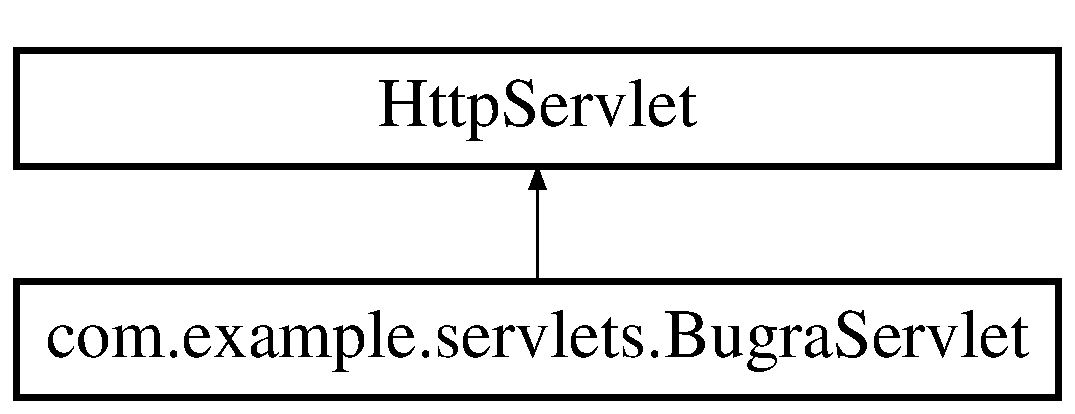
\includegraphics[height=2.000000cm]{classcom_1_1example_1_1servlets_1_1_bugra_servlet}
\end{center}
\end{figure}
\subsection*{Public Member Functions}
\begin{DoxyCompactItemize}
\item 
\hyperlink{classcom_1_1example_1_1servlets_1_1_bugra_servlet_a99bb8aae42b1719184ea8c7d9fee9030}{Bugra\+Servlet} ()
\end{DoxyCompactItemize}
\subsection*{Protected Member Functions}
\begin{DoxyCompactItemize}
\item 
void \hyperlink{classcom_1_1example_1_1servlets_1_1_bugra_servlet_a0874481d6101ca58a052edeb9ce9a815}{do\+Get} (Http\+Servlet\+Request request, Http\+Servlet\+Response response)  throws Servlet\+Exception, I\+O\+Exception 
\item 
void \hyperlink{classcom_1_1example_1_1servlets_1_1_bugra_servlet_a049250502b8d42e00612a0e249b8e3e2}{do\+Post} (Http\+Servlet\+Request request, Http\+Servlet\+Response response)  throws Servlet\+Exception, I\+O\+Exception 
\end{DoxyCompactItemize}
\subsection*{Static Private Attributes}
\begin{DoxyCompactItemize}
\item 
static final long \hyperlink{classcom_1_1example_1_1servlets_1_1_bugra_servlet_a017b832dab85959c1a172b508ce28716}{serial\+Version\+U\+ID} = 1L
\end{DoxyCompactItemize}


\subsection{Detailed Description}
Servlet implementation class \hyperlink{classcom_1_1example_1_1servlets_1_1_bugra_servlet}{Bugra\+Servlet} 

\subsection{Constructor \& Destructor Documentation}
\index{com\+::example\+::servlets\+::\+Bugra\+Servlet@{com\+::example\+::servlets\+::\+Bugra\+Servlet}!Bugra\+Servlet@{Bugra\+Servlet}}
\index{Bugra\+Servlet@{Bugra\+Servlet}!com\+::example\+::servlets\+::\+Bugra\+Servlet@{com\+::example\+::servlets\+::\+Bugra\+Servlet}}
\subsubsection[{\texorpdfstring{Bugra\+Servlet()}{BugraServlet()}}]{\setlength{\rightskip}{0pt plus 5cm}com.\+example.\+servlets.\+Bugra\+Servlet.\+Bugra\+Servlet (
\begin{DoxyParamCaption}
{}
\end{DoxyParamCaption}
)}\hypertarget{classcom_1_1example_1_1servlets_1_1_bugra_servlet_a99bb8aae42b1719184ea8c7d9fee9030}{}\label{classcom_1_1example_1_1servlets_1_1_bugra_servlet_a99bb8aae42b1719184ea8c7d9fee9030}
Default constructor. 

\subsection{Member Function Documentation}
\index{com\+::example\+::servlets\+::\+Bugra\+Servlet@{com\+::example\+::servlets\+::\+Bugra\+Servlet}!do\+Get@{do\+Get}}
\index{do\+Get@{do\+Get}!com\+::example\+::servlets\+::\+Bugra\+Servlet@{com\+::example\+::servlets\+::\+Bugra\+Servlet}}
\subsubsection[{\texorpdfstring{do\+Get(\+Http\+Servlet\+Request request, Http\+Servlet\+Response response)}{doGet(HttpServletRequest request, HttpServletResponse response)}}]{\setlength{\rightskip}{0pt plus 5cm}void com.\+example.\+servlets.\+Bugra\+Servlet.\+do\+Get (
\begin{DoxyParamCaption}
\item[{Http\+Servlet\+Request}]{request, }
\item[{Http\+Servlet\+Response}]{response}
\end{DoxyParamCaption}
) throws Servlet\+Exception, I\+O\+Exception\hspace{0.3cm}{\ttfamily [protected]}}\hypertarget{classcom_1_1example_1_1servlets_1_1_bugra_servlet_a0874481d6101ca58a052edeb9ce9a815}{}\label{classcom_1_1example_1_1servlets_1_1_bugra_servlet_a0874481d6101ca58a052edeb9ce9a815}
\begin{DoxySeeAlso}{See also}
Http\+Servlet\+::do\+Get(\+Http\+Servlet\+Request request, Http\+Servlet\+Response response) 
\end{DoxySeeAlso}
\index{com\+::example\+::servlets\+::\+Bugra\+Servlet@{com\+::example\+::servlets\+::\+Bugra\+Servlet}!do\+Post@{do\+Post}}
\index{do\+Post@{do\+Post}!com\+::example\+::servlets\+::\+Bugra\+Servlet@{com\+::example\+::servlets\+::\+Bugra\+Servlet}}
\subsubsection[{\texorpdfstring{do\+Post(\+Http\+Servlet\+Request request, Http\+Servlet\+Response response)}{doPost(HttpServletRequest request, HttpServletResponse response)}}]{\setlength{\rightskip}{0pt plus 5cm}void com.\+example.\+servlets.\+Bugra\+Servlet.\+do\+Post (
\begin{DoxyParamCaption}
\item[{Http\+Servlet\+Request}]{request, }
\item[{Http\+Servlet\+Response}]{response}
\end{DoxyParamCaption}
) throws Servlet\+Exception, I\+O\+Exception\hspace{0.3cm}{\ttfamily [protected]}}\hypertarget{classcom_1_1example_1_1servlets_1_1_bugra_servlet_a049250502b8d42e00612a0e249b8e3e2}{}\label{classcom_1_1example_1_1servlets_1_1_bugra_servlet_a049250502b8d42e00612a0e249b8e3e2}
\begin{DoxySeeAlso}{See also}
Http\+Servlet\+::do\+Post(\+Http\+Servlet\+Request request, Http\+Servlet\+Response response) 
\end{DoxySeeAlso}


\subsection{Member Data Documentation}
\index{com\+::example\+::servlets\+::\+Bugra\+Servlet@{com\+::example\+::servlets\+::\+Bugra\+Servlet}!serial\+Version\+U\+ID@{serial\+Version\+U\+ID}}
\index{serial\+Version\+U\+ID@{serial\+Version\+U\+ID}!com\+::example\+::servlets\+::\+Bugra\+Servlet@{com\+::example\+::servlets\+::\+Bugra\+Servlet}}
\subsubsection[{\texorpdfstring{serial\+Version\+U\+ID}{serialVersionUID}}]{\setlength{\rightskip}{0pt plus 5cm}final long com.\+example.\+servlets.\+Bugra\+Servlet.\+serial\+Version\+U\+ID = 1L\hspace{0.3cm}{\ttfamily [static]}, {\ttfamily [private]}}\hypertarget{classcom_1_1example_1_1servlets_1_1_bugra_servlet_a017b832dab85959c1a172b508ce28716}{}\label{classcom_1_1example_1_1servlets_1_1_bugra_servlet_a017b832dab85959c1a172b508ce28716}


The documentation for this class was generated from the following file\+:\begin{DoxyCompactItemize}
\item 
src/com/example/servlets/\hyperlink{_bugra_servlet_8java}{Bugra\+Servlet.\+java}\end{DoxyCompactItemize}

\hypertarget{classcom_1_1example_1_1servlets_1_1_burak_servlet}{}\section{com.\+example.\+servlets.\+Burak\+Servlet Class Reference}
\label{classcom_1_1example_1_1servlets_1_1_burak_servlet}\index{com.\+example.\+servlets.\+Burak\+Servlet@{com.\+example.\+servlets.\+Burak\+Servlet}}
Inheritance diagram for com.\+example.\+servlets.\+Burak\+Servlet\+:\begin{figure}[H]
\begin{center}
\leavevmode
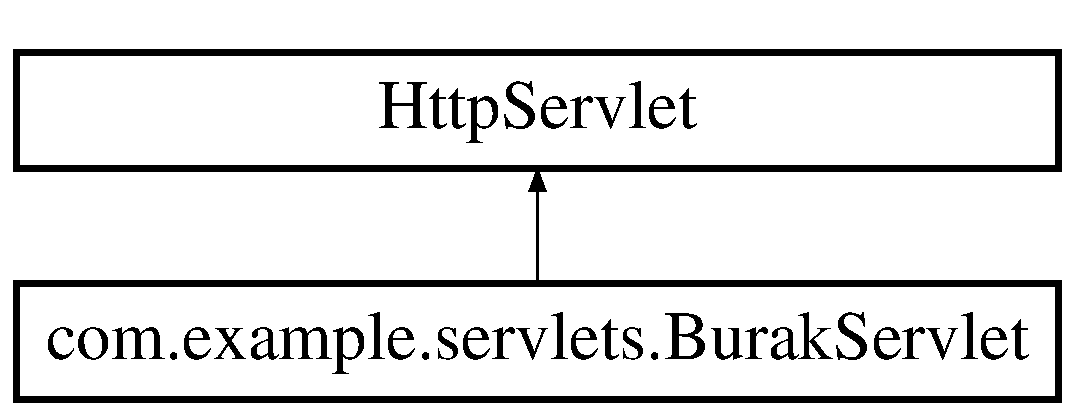
\includegraphics[height=2.000000cm]{classcom_1_1example_1_1servlets_1_1_burak_servlet}
\end{center}
\end{figure}
\subsection*{Public Member Functions}
\begin{DoxyCompactItemize}
\item 
\hyperlink{classcom_1_1example_1_1servlets_1_1_burak_servlet_a933d316f89b292a7b8d4b84fdd551d45}{Burak\+Servlet} ()
\end{DoxyCompactItemize}
\subsection*{Protected Member Functions}
\begin{DoxyCompactItemize}
\item 
void \hyperlink{classcom_1_1example_1_1servlets_1_1_burak_servlet_afad2ce1980f63c828bcb6bb420276477}{do\+Get} (Http\+Servlet\+Request request, Http\+Servlet\+Response response)  throws Servlet\+Exception, I\+O\+Exception 
\item 
void \hyperlink{classcom_1_1example_1_1servlets_1_1_burak_servlet_ae2d3d9cb85c12eef39cd2145baaf75ef}{do\+Post} (Http\+Servlet\+Request request, Http\+Servlet\+Response response)  throws Servlet\+Exception, I\+O\+Exception 
\end{DoxyCompactItemize}
\subsection*{Static Private Attributes}
\begin{DoxyCompactItemize}
\item 
static final long \hyperlink{classcom_1_1example_1_1servlets_1_1_burak_servlet_a03b3133becc008e75537df6820aaef5c}{serial\+Version\+U\+ID} = 1L
\end{DoxyCompactItemize}


\subsection{Detailed Description}
Servlet implementation class \hyperlink{classcom_1_1example_1_1servlets_1_1_burak_servlet}{Burak\+Servlet} 

\subsection{Constructor \& Destructor Documentation}
\index{com\+::example\+::servlets\+::\+Burak\+Servlet@{com\+::example\+::servlets\+::\+Burak\+Servlet}!Burak\+Servlet@{Burak\+Servlet}}
\index{Burak\+Servlet@{Burak\+Servlet}!com\+::example\+::servlets\+::\+Burak\+Servlet@{com\+::example\+::servlets\+::\+Burak\+Servlet}}
\subsubsection[{\texorpdfstring{Burak\+Servlet()}{BurakServlet()}}]{\setlength{\rightskip}{0pt plus 5cm}com.\+example.\+servlets.\+Burak\+Servlet.\+Burak\+Servlet (
\begin{DoxyParamCaption}
{}
\end{DoxyParamCaption}
)}\hypertarget{classcom_1_1example_1_1servlets_1_1_burak_servlet_a933d316f89b292a7b8d4b84fdd551d45}{}\label{classcom_1_1example_1_1servlets_1_1_burak_servlet_a933d316f89b292a7b8d4b84fdd551d45}
\begin{DoxySeeAlso}{See also}
Http\+Servlet\+::\+Http\+Servlet() 
\end{DoxySeeAlso}


\subsection{Member Function Documentation}
\index{com\+::example\+::servlets\+::\+Burak\+Servlet@{com\+::example\+::servlets\+::\+Burak\+Servlet}!do\+Get@{do\+Get}}
\index{do\+Get@{do\+Get}!com\+::example\+::servlets\+::\+Burak\+Servlet@{com\+::example\+::servlets\+::\+Burak\+Servlet}}
\subsubsection[{\texorpdfstring{do\+Get(\+Http\+Servlet\+Request request, Http\+Servlet\+Response response)}{doGet(HttpServletRequest request, HttpServletResponse response)}}]{\setlength{\rightskip}{0pt plus 5cm}void com.\+example.\+servlets.\+Burak\+Servlet.\+do\+Get (
\begin{DoxyParamCaption}
\item[{Http\+Servlet\+Request}]{request, }
\item[{Http\+Servlet\+Response}]{response}
\end{DoxyParamCaption}
) throws Servlet\+Exception, I\+O\+Exception\hspace{0.3cm}{\ttfamily [protected]}}\hypertarget{classcom_1_1example_1_1servlets_1_1_burak_servlet_afad2ce1980f63c828bcb6bb420276477}{}\label{classcom_1_1example_1_1servlets_1_1_burak_servlet_afad2ce1980f63c828bcb6bb420276477}
\begin{DoxySeeAlso}{See also}
Http\+Servlet\+::do\+Get(\+Http\+Servlet\+Request request, Http\+Servlet\+Response response) 
\end{DoxySeeAlso}
\index{com\+::example\+::servlets\+::\+Burak\+Servlet@{com\+::example\+::servlets\+::\+Burak\+Servlet}!do\+Post@{do\+Post}}
\index{do\+Post@{do\+Post}!com\+::example\+::servlets\+::\+Burak\+Servlet@{com\+::example\+::servlets\+::\+Burak\+Servlet}}
\subsubsection[{\texorpdfstring{do\+Post(\+Http\+Servlet\+Request request, Http\+Servlet\+Response response)}{doPost(HttpServletRequest request, HttpServletResponse response)}}]{\setlength{\rightskip}{0pt plus 5cm}void com.\+example.\+servlets.\+Burak\+Servlet.\+do\+Post (
\begin{DoxyParamCaption}
\item[{Http\+Servlet\+Request}]{request, }
\item[{Http\+Servlet\+Response}]{response}
\end{DoxyParamCaption}
) throws Servlet\+Exception, I\+O\+Exception\hspace{0.3cm}{\ttfamily [protected]}}\hypertarget{classcom_1_1example_1_1servlets_1_1_burak_servlet_ae2d3d9cb85c12eef39cd2145baaf75ef}{}\label{classcom_1_1example_1_1servlets_1_1_burak_servlet_ae2d3d9cb85c12eef39cd2145baaf75ef}
\begin{DoxySeeAlso}{See also}
Http\+Servlet\+::do\+Post(\+Http\+Servlet\+Request request, Http\+Servlet\+Response response) 
\end{DoxySeeAlso}


\subsection{Member Data Documentation}
\index{com\+::example\+::servlets\+::\+Burak\+Servlet@{com\+::example\+::servlets\+::\+Burak\+Servlet}!serial\+Version\+U\+ID@{serial\+Version\+U\+ID}}
\index{serial\+Version\+U\+ID@{serial\+Version\+U\+ID}!com\+::example\+::servlets\+::\+Burak\+Servlet@{com\+::example\+::servlets\+::\+Burak\+Servlet}}
\subsubsection[{\texorpdfstring{serial\+Version\+U\+ID}{serialVersionUID}}]{\setlength{\rightskip}{0pt plus 5cm}final long com.\+example.\+servlets.\+Burak\+Servlet.\+serial\+Version\+U\+ID = 1L\hspace{0.3cm}{\ttfamily [static]}, {\ttfamily [private]}}\hypertarget{classcom_1_1example_1_1servlets_1_1_burak_servlet_a03b3133becc008e75537df6820aaef5c}{}\label{classcom_1_1example_1_1servlets_1_1_burak_servlet_a03b3133becc008e75537df6820aaef5c}


The documentation for this class was generated from the following file\+:\begin{DoxyCompactItemize}
\item 
src/com/example/servlets/\hyperlink{_burak_servlet_8java}{Burak\+Servlet.\+java}\end{DoxyCompactItemize}

\hypertarget{classcom_1_1example_1_1servlets_1_1_hello_servlet}{}\section{com.\+example.\+servlets.\+Hello\+Servlet Class Reference}
\label{classcom_1_1example_1_1servlets_1_1_hello_servlet}\index{com.\+example.\+servlets.\+Hello\+Servlet@{com.\+example.\+servlets.\+Hello\+Servlet}}
Inheritance diagram for com.\+example.\+servlets.\+Hello\+Servlet\+:\begin{figure}[H]
\begin{center}
\leavevmode
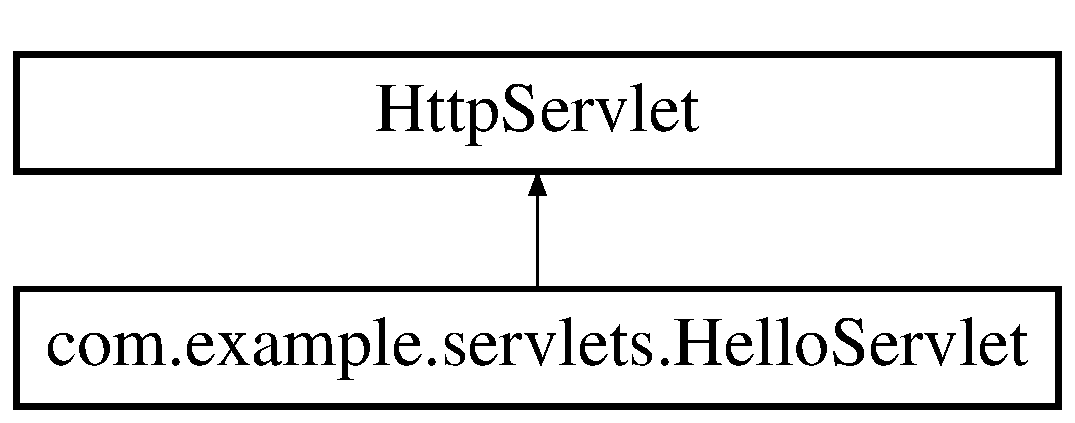
\includegraphics[height=2.000000cm]{classcom_1_1example_1_1servlets_1_1_hello_servlet}
\end{center}
\end{figure}
\subsection*{Public Member Functions}
\begin{DoxyCompactItemize}
\item 
\hyperlink{classcom_1_1example_1_1servlets_1_1_hello_servlet_acde0125d36d0d4cbbe7ed5d5ccc93c54}{Hello\+Servlet} ()
\end{DoxyCompactItemize}
\subsection*{Protected Member Functions}
\begin{DoxyCompactItemize}
\item 
void \hyperlink{classcom_1_1example_1_1servlets_1_1_hello_servlet_aebf5d769bdf4e1181b45c870ee9d9c49}{do\+Get} (Http\+Servlet\+Request request, Http\+Servlet\+Response response)  throws Servlet\+Exception, I\+O\+Exception 
\item 
void \hyperlink{classcom_1_1example_1_1servlets_1_1_hello_servlet_add7f3c9daaaccbe81fe119dd8ae99ae4}{do\+Post} (Http\+Servlet\+Request request, Http\+Servlet\+Response response)  throws Servlet\+Exception, I\+O\+Exception 
\end{DoxyCompactItemize}
\subsection*{Static Private Attributes}
\begin{DoxyCompactItemize}
\item 
static final long \hyperlink{classcom_1_1example_1_1servlets_1_1_hello_servlet_aee3a8f698be2149a6d0c401ab648cf82}{serial\+Version\+U\+I\+D} = 1\+L
\end{DoxyCompactItemize}


\subsection{Detailed Description}
Servlet implementation class \hyperlink{classcom_1_1example_1_1servlets_1_1_hello_servlet}{Hello\+Servlet} 

\subsection{Constructor \& Destructor Documentation}
\hypertarget{classcom_1_1example_1_1servlets_1_1_hello_servlet_acde0125d36d0d4cbbe7ed5d5ccc93c54}{}\index{com\+::example\+::servlets\+::\+Hello\+Servlet@{com\+::example\+::servlets\+::\+Hello\+Servlet}!Hello\+Servlet@{Hello\+Servlet}}
\index{Hello\+Servlet@{Hello\+Servlet}!com\+::example\+::servlets\+::\+Hello\+Servlet@{com\+::example\+::servlets\+::\+Hello\+Servlet}}
\subsubsection[{Hello\+Servlet()}]{\setlength{\rightskip}{0pt plus 5cm}com.\+example.\+servlets.\+Hello\+Servlet.\+Hello\+Servlet (
\begin{DoxyParamCaption}
{}
\end{DoxyParamCaption}
)}\label{classcom_1_1example_1_1servlets_1_1_hello_servlet_acde0125d36d0d4cbbe7ed5d5ccc93c54}
\begin{DoxySeeAlso}{See also}
Http\+Servlet\+::\+Http\+Servlet() 
\end{DoxySeeAlso}


\subsection{Member Function Documentation}
\hypertarget{classcom_1_1example_1_1servlets_1_1_hello_servlet_aebf5d769bdf4e1181b45c870ee9d9c49}{}\index{com\+::example\+::servlets\+::\+Hello\+Servlet@{com\+::example\+::servlets\+::\+Hello\+Servlet}!do\+Get@{do\+Get}}
\index{do\+Get@{do\+Get}!com\+::example\+::servlets\+::\+Hello\+Servlet@{com\+::example\+::servlets\+::\+Hello\+Servlet}}
\subsubsection[{do\+Get(\+Http\+Servlet\+Request request, Http\+Servlet\+Response response)}]{\setlength{\rightskip}{0pt plus 5cm}void com.\+example.\+servlets.\+Hello\+Servlet.\+do\+Get (
\begin{DoxyParamCaption}
\item[{Http\+Servlet\+Request}]{request, }
\item[{Http\+Servlet\+Response}]{response}
\end{DoxyParamCaption}
) throws Servlet\+Exception, I\+O\+Exception\hspace{0.3cm}{\ttfamily [protected]}}\label{classcom_1_1example_1_1servlets_1_1_hello_servlet_aebf5d769bdf4e1181b45c870ee9d9c49}
\begin{DoxySeeAlso}{See also}
Http\+Servlet\+::do\+Get(\+Http\+Servlet\+Request request, Http\+Servlet\+Response response) 
\end{DoxySeeAlso}
\hypertarget{classcom_1_1example_1_1servlets_1_1_hello_servlet_add7f3c9daaaccbe81fe119dd8ae99ae4}{}\index{com\+::example\+::servlets\+::\+Hello\+Servlet@{com\+::example\+::servlets\+::\+Hello\+Servlet}!do\+Post@{do\+Post}}
\index{do\+Post@{do\+Post}!com\+::example\+::servlets\+::\+Hello\+Servlet@{com\+::example\+::servlets\+::\+Hello\+Servlet}}
\subsubsection[{do\+Post(\+Http\+Servlet\+Request request, Http\+Servlet\+Response response)}]{\setlength{\rightskip}{0pt plus 5cm}void com.\+example.\+servlets.\+Hello\+Servlet.\+do\+Post (
\begin{DoxyParamCaption}
\item[{Http\+Servlet\+Request}]{request, }
\item[{Http\+Servlet\+Response}]{response}
\end{DoxyParamCaption}
) throws Servlet\+Exception, I\+O\+Exception\hspace{0.3cm}{\ttfamily [protected]}}\label{classcom_1_1example_1_1servlets_1_1_hello_servlet_add7f3c9daaaccbe81fe119dd8ae99ae4}
\begin{DoxySeeAlso}{See also}
Http\+Servlet\+::do\+Post(\+Http\+Servlet\+Request request, Http\+Servlet\+Response response) 
\end{DoxySeeAlso}


\subsection{Member Data Documentation}
\hypertarget{classcom_1_1example_1_1servlets_1_1_hello_servlet_aee3a8f698be2149a6d0c401ab648cf82}{}\index{com\+::example\+::servlets\+::\+Hello\+Servlet@{com\+::example\+::servlets\+::\+Hello\+Servlet}!serial\+Version\+U\+I\+D@{serial\+Version\+U\+I\+D}}
\index{serial\+Version\+U\+I\+D@{serial\+Version\+U\+I\+D}!com\+::example\+::servlets\+::\+Hello\+Servlet@{com\+::example\+::servlets\+::\+Hello\+Servlet}}
\subsubsection[{serial\+Version\+U\+I\+D}]{\setlength{\rightskip}{0pt plus 5cm}final long com.\+example.\+servlets.\+Hello\+Servlet.\+serial\+Version\+U\+I\+D = 1\+L\hspace{0.3cm}{\ttfamily [static]}, {\ttfamily [private]}}\label{classcom_1_1example_1_1servlets_1_1_hello_servlet_aee3a8f698be2149a6d0c401ab648cf82}


The documentation for this class was generated from the following file\+:\begin{DoxyCompactItemize}
\item 
src/com/example/servlets/\hyperlink{_hello_servlet_8java}{Hello\+Servlet.\+java}\end{DoxyCompactItemize}

\hypertarget{classcom_1_1example_1_1servlets_1_1_kerim_servlet}{}\section{com.\+example.\+servlets.\+Kerim\+Servlet Class Reference}
\label{classcom_1_1example_1_1servlets_1_1_kerim_servlet}\index{com.\+example.\+servlets.\+Kerim\+Servlet@{com.\+example.\+servlets.\+Kerim\+Servlet}}


This class is written for the personal assignment 6.  


Inheritance diagram for com.\+example.\+servlets.\+Kerim\+Servlet\+:\begin{figure}[H]
\begin{center}
\leavevmode
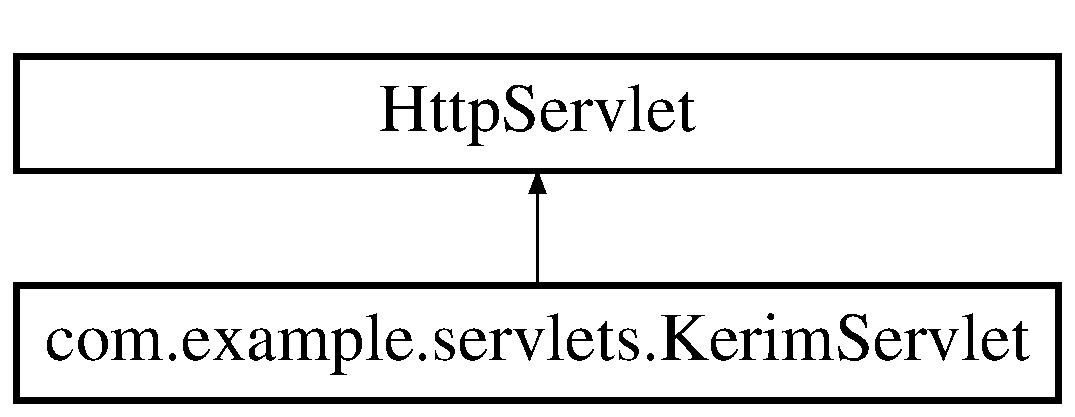
\includegraphics[height=2.000000cm]{classcom_1_1example_1_1servlets_1_1_kerim_servlet}
\end{center}
\end{figure}
\subsection*{Public Member Functions}
\begin{DoxyCompactItemize}
\item 
Connection \hyperlink{classcom_1_1example_1_1servlets_1_1_kerim_servlet_a3668be62679c5fd89eda37828b156fbb}{mysql\+Connection} ()
\begin{DoxyCompactList}\small\item\em Connects to database and returns the connection handle. \end{DoxyCompactList}\item 
\hyperlink{classcom_1_1example_1_1servlets_1_1_kerim_servlet_ab507212f5e073be787370e98807d881a}{Kerim\+Servlet} ()
\begin{DoxyCompactList}\small\item\em The constructor calls the superclass constructor. \end{DoxyCompactList}\end{DoxyCompactItemize}
\subsection*{Protected Member Functions}
\begin{DoxyCompactItemize}
\item 
void \hyperlink{classcom_1_1example_1_1servlets_1_1_kerim_servlet_add82d54e7368760364154a77773395fb}{do\+Get} (Http\+Servlet\+Request req, Http\+Servlet\+Response resp)  throws Servlet\+Exception, I\+O\+Exception 
\item 
void \hyperlink{classcom_1_1example_1_1servlets_1_1_kerim_servlet_ac8c55b1078359fa7c06e63694eb06377}{do\+Post} (Http\+Servlet\+Request req, Http\+Servlet\+Response resp)  throws Servlet\+Exception, I\+O\+Exception 
\end{DoxyCompactItemize}
\subsection*{Static Private Attributes}
\begin{DoxyCompactItemize}
\item 
static final long \hyperlink{classcom_1_1example_1_1servlets_1_1_kerim_servlet_a659a1f9d230ee60ab4f87c1f95d34ab9}{serial\+Version\+U\+I\+D} = 3818282702335774732\+L
\end{DoxyCompactItemize}


\subsection{Detailed Description}
This class is written for the personal assignment 6. 

\begin{DoxyAuthor}{Author}
kerimgokarslan Kerim Gokarslan\href{mailto:kerim.gokarslan@boun.edu.tr}{\tt kerim.\+gokarslan@boun.\+edu.\+tr} 2012400030 This code is written for the assignment 6 of the course Cmp\+E 352 Spring \textquotesingle{}16. version 1.\+0 
\end{DoxyAuthor}


\subsection{Constructor \& Destructor Documentation}
\hypertarget{classcom_1_1example_1_1servlets_1_1_kerim_servlet_ab507212f5e073be787370e98807d881a}{}\index{com\+::example\+::servlets\+::\+Kerim\+Servlet@{com\+::example\+::servlets\+::\+Kerim\+Servlet}!Kerim\+Servlet@{Kerim\+Servlet}}
\index{Kerim\+Servlet@{Kerim\+Servlet}!com\+::example\+::servlets\+::\+Kerim\+Servlet@{com\+::example\+::servlets\+::\+Kerim\+Servlet}}
\subsubsection[{Kerim\+Servlet()}]{\setlength{\rightskip}{0pt plus 5cm}com.\+example.\+servlets.\+Kerim\+Servlet.\+Kerim\+Servlet (
\begin{DoxyParamCaption}
{}
\end{DoxyParamCaption}
)}\label{classcom_1_1example_1_1servlets_1_1_kerim_servlet_ab507212f5e073be787370e98807d881a}


The constructor calls the superclass constructor. 



\subsection{Member Function Documentation}
\hypertarget{classcom_1_1example_1_1servlets_1_1_kerim_servlet_add82d54e7368760364154a77773395fb}{}\index{com\+::example\+::servlets\+::\+Kerim\+Servlet@{com\+::example\+::servlets\+::\+Kerim\+Servlet}!do\+Get@{do\+Get}}
\index{do\+Get@{do\+Get}!com\+::example\+::servlets\+::\+Kerim\+Servlet@{com\+::example\+::servlets\+::\+Kerim\+Servlet}}
\subsubsection[{do\+Get(\+Http\+Servlet\+Request req, Http\+Servlet\+Response resp)}]{\setlength{\rightskip}{0pt plus 5cm}void com.\+example.\+servlets.\+Kerim\+Servlet.\+do\+Get (
\begin{DoxyParamCaption}
\item[{Http\+Servlet\+Request}]{req, }
\item[{Http\+Servlet\+Response}]{resp}
\end{DoxyParamCaption}
) throws Servlet\+Exception, I\+O\+Exception\hspace{0.3cm}{\ttfamily [protected]}}\label{classcom_1_1example_1_1servlets_1_1_kerim_servlet_add82d54e7368760364154a77773395fb}
\hypertarget{classcom_1_1example_1_1servlets_1_1_kerim_servlet_ac8c55b1078359fa7c06e63694eb06377}{}\index{com\+::example\+::servlets\+::\+Kerim\+Servlet@{com\+::example\+::servlets\+::\+Kerim\+Servlet}!do\+Post@{do\+Post}}
\index{do\+Post@{do\+Post}!com\+::example\+::servlets\+::\+Kerim\+Servlet@{com\+::example\+::servlets\+::\+Kerim\+Servlet}}
\subsubsection[{do\+Post(\+Http\+Servlet\+Request req, Http\+Servlet\+Response resp)}]{\setlength{\rightskip}{0pt plus 5cm}void com.\+example.\+servlets.\+Kerim\+Servlet.\+do\+Post (
\begin{DoxyParamCaption}
\item[{Http\+Servlet\+Request}]{req, }
\item[{Http\+Servlet\+Response}]{resp}
\end{DoxyParamCaption}
) throws Servlet\+Exception, I\+O\+Exception\hspace{0.3cm}{\ttfamily [protected]}}\label{classcom_1_1example_1_1servlets_1_1_kerim_servlet_ac8c55b1078359fa7c06e63694eb06377}
\hypertarget{classcom_1_1example_1_1servlets_1_1_kerim_servlet_a3668be62679c5fd89eda37828b156fbb}{}\index{com\+::example\+::servlets\+::\+Kerim\+Servlet@{com\+::example\+::servlets\+::\+Kerim\+Servlet}!mysql\+Connection@{mysql\+Connection}}
\index{mysql\+Connection@{mysql\+Connection}!com\+::example\+::servlets\+::\+Kerim\+Servlet@{com\+::example\+::servlets\+::\+Kerim\+Servlet}}
\subsubsection[{mysql\+Connection()}]{\setlength{\rightskip}{0pt plus 5cm}Connection com.\+example.\+servlets.\+Kerim\+Servlet.\+mysql\+Connection (
\begin{DoxyParamCaption}
{}
\end{DoxyParamCaption}
)}\label{classcom_1_1example_1_1servlets_1_1_kerim_servlet_a3668be62679c5fd89eda37828b156fbb}


Connects to database and returns the connection handle. 

\begin{DoxyReturn}{Returns}

\end{DoxyReturn}


\subsection{Member Data Documentation}
\hypertarget{classcom_1_1example_1_1servlets_1_1_kerim_servlet_a659a1f9d230ee60ab4f87c1f95d34ab9}{}\index{com\+::example\+::servlets\+::\+Kerim\+Servlet@{com\+::example\+::servlets\+::\+Kerim\+Servlet}!serial\+Version\+U\+I\+D@{serial\+Version\+U\+I\+D}}
\index{serial\+Version\+U\+I\+D@{serial\+Version\+U\+I\+D}!com\+::example\+::servlets\+::\+Kerim\+Servlet@{com\+::example\+::servlets\+::\+Kerim\+Servlet}}
\subsubsection[{serial\+Version\+U\+I\+D}]{\setlength{\rightskip}{0pt plus 5cm}final long com.\+example.\+servlets.\+Kerim\+Servlet.\+serial\+Version\+U\+I\+D = 3818282702335774732\+L\hspace{0.3cm}{\ttfamily [static]}, {\ttfamily [private]}}\label{classcom_1_1example_1_1servlets_1_1_kerim_servlet_a659a1f9d230ee60ab4f87c1f95d34ab9}


The documentation for this class was generated from the following file\+:\begin{DoxyCompactItemize}
\item 
src/com/example/servlets/\hyperlink{_kerim_servlet_8java}{Kerim\+Servlet.\+java}\end{DoxyCompactItemize}

\hypertarget{classcom_1_1example_1_1servlets_1_1_ozer2_servlet}{}\section{com.\+example.\+servlets.\+Ozer2\+Servlet Class Reference}
\label{classcom_1_1example_1_1servlets_1_1_ozer2_servlet}\index{com.\+example.\+servlets.\+Ozer2\+Servlet@{com.\+example.\+servlets.\+Ozer2\+Servlet}}
Inheritance diagram for com.\+example.\+servlets.\+Ozer2\+Servlet\+:\begin{figure}[H]
\begin{center}
\leavevmode
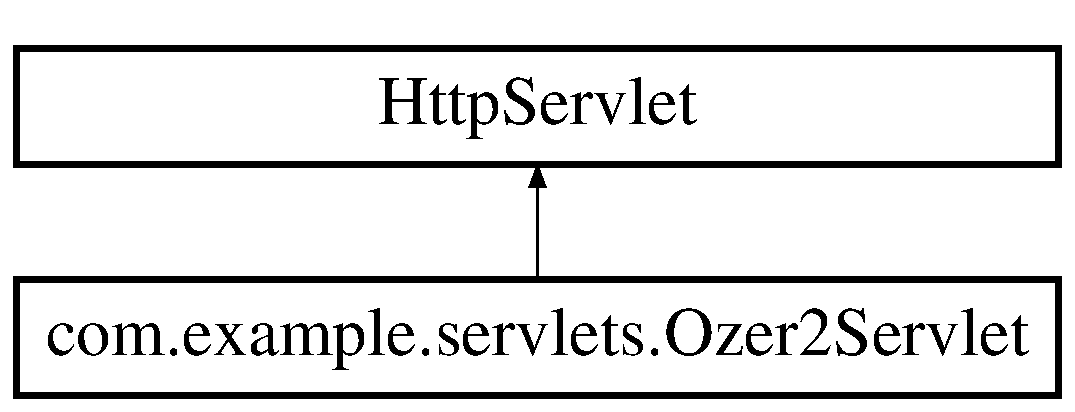
\includegraphics[height=2.000000cm]{classcom_1_1example_1_1servlets_1_1_ozer2_servlet}
\end{center}
\end{figure}
\subsection*{Public Member Functions}
\begin{DoxyCompactItemize}
\item 
\hyperlink{classcom_1_1example_1_1servlets_1_1_ozer2_servlet_a06251df51ea525cfedf5dec488ad58f2}{Ozer2\+Servlet} ()
\end{DoxyCompactItemize}
\subsection*{Protected Member Functions}
\begin{DoxyCompactItemize}
\item 
void \hyperlink{classcom_1_1example_1_1servlets_1_1_ozer2_servlet_af9ddf218ed38e3372658be9ebfbdde64}{do\+Get} (Http\+Servlet\+Request request, Http\+Servlet\+Response response)  throws Servlet\+Exception, I\+O\+Exception 
\item 
void \hyperlink{classcom_1_1example_1_1servlets_1_1_ozer2_servlet_a3dc6ef2c0365fad91e8ebb6b9106551a}{do\+Post} (Http\+Servlet\+Request request, Http\+Servlet\+Response response)  throws Servlet\+Exception, I\+O\+Exception 
\end{DoxyCompactItemize}
\subsection*{Static Private Attributes}
\begin{DoxyCompactItemize}
\item 
static final long \hyperlink{classcom_1_1example_1_1servlets_1_1_ozer2_servlet_adda557e8b6e5941a32e2aa6a66ad1295}{serial\+Version\+U\+ID} = 1L
\end{DoxyCompactItemize}


\subsection{Detailed Description}
Servlet implementation class \hyperlink{classcom_1_1example_1_1servlets_1_1_ozer2_servlet}{Ozer2\+Servlet} 

\subsection{Constructor \& Destructor Documentation}
\index{com\+::example\+::servlets\+::\+Ozer2\+Servlet@{com\+::example\+::servlets\+::\+Ozer2\+Servlet}!Ozer2\+Servlet@{Ozer2\+Servlet}}
\index{Ozer2\+Servlet@{Ozer2\+Servlet}!com\+::example\+::servlets\+::\+Ozer2\+Servlet@{com\+::example\+::servlets\+::\+Ozer2\+Servlet}}
\subsubsection[{\texorpdfstring{Ozer2\+Servlet()}{Ozer2Servlet()}}]{\setlength{\rightskip}{0pt plus 5cm}com.\+example.\+servlets.\+Ozer2\+Servlet.\+Ozer2\+Servlet (
\begin{DoxyParamCaption}
{}
\end{DoxyParamCaption}
)}\hypertarget{classcom_1_1example_1_1servlets_1_1_ozer2_servlet_a06251df51ea525cfedf5dec488ad58f2}{}\label{classcom_1_1example_1_1servlets_1_1_ozer2_servlet_a06251df51ea525cfedf5dec488ad58f2}
\begin{DoxySeeAlso}{See also}
Http\+Servlet\+::\+Http\+Servlet() 
\end{DoxySeeAlso}


\subsection{Member Function Documentation}
\index{com\+::example\+::servlets\+::\+Ozer2\+Servlet@{com\+::example\+::servlets\+::\+Ozer2\+Servlet}!do\+Get@{do\+Get}}
\index{do\+Get@{do\+Get}!com\+::example\+::servlets\+::\+Ozer2\+Servlet@{com\+::example\+::servlets\+::\+Ozer2\+Servlet}}
\subsubsection[{\texorpdfstring{do\+Get(\+Http\+Servlet\+Request request, Http\+Servlet\+Response response)}{doGet(HttpServletRequest request, HttpServletResponse response)}}]{\setlength{\rightskip}{0pt plus 5cm}void com.\+example.\+servlets.\+Ozer2\+Servlet.\+do\+Get (
\begin{DoxyParamCaption}
\item[{Http\+Servlet\+Request}]{request, }
\item[{Http\+Servlet\+Response}]{response}
\end{DoxyParamCaption}
) throws Servlet\+Exception, I\+O\+Exception\hspace{0.3cm}{\ttfamily [protected]}}\hypertarget{classcom_1_1example_1_1servlets_1_1_ozer2_servlet_af9ddf218ed38e3372658be9ebfbdde64}{}\label{classcom_1_1example_1_1servlets_1_1_ozer2_servlet_af9ddf218ed38e3372658be9ebfbdde64}
\begin{DoxySeeAlso}{See also}
Http\+Servlet\+::do\+Get(\+Http\+Servlet\+Request request, Http\+Servlet\+Response response) 
\end{DoxySeeAlso}
\index{com\+::example\+::servlets\+::\+Ozer2\+Servlet@{com\+::example\+::servlets\+::\+Ozer2\+Servlet}!do\+Post@{do\+Post}}
\index{do\+Post@{do\+Post}!com\+::example\+::servlets\+::\+Ozer2\+Servlet@{com\+::example\+::servlets\+::\+Ozer2\+Servlet}}
\subsubsection[{\texorpdfstring{do\+Post(\+Http\+Servlet\+Request request, Http\+Servlet\+Response response)}{doPost(HttpServletRequest request, HttpServletResponse response)}}]{\setlength{\rightskip}{0pt plus 5cm}void com.\+example.\+servlets.\+Ozer2\+Servlet.\+do\+Post (
\begin{DoxyParamCaption}
\item[{Http\+Servlet\+Request}]{request, }
\item[{Http\+Servlet\+Response}]{response}
\end{DoxyParamCaption}
) throws Servlet\+Exception, I\+O\+Exception\hspace{0.3cm}{\ttfamily [protected]}}\hypertarget{classcom_1_1example_1_1servlets_1_1_ozer2_servlet_a3dc6ef2c0365fad91e8ebb6b9106551a}{}\label{classcom_1_1example_1_1servlets_1_1_ozer2_servlet_a3dc6ef2c0365fad91e8ebb6b9106551a}
\begin{DoxySeeAlso}{See also}
Http\+Servlet\+::do\+Post(\+Http\+Servlet\+Request request, Http\+Servlet\+Response response) 
\end{DoxySeeAlso}


\subsection{Member Data Documentation}
\index{com\+::example\+::servlets\+::\+Ozer2\+Servlet@{com\+::example\+::servlets\+::\+Ozer2\+Servlet}!serial\+Version\+U\+ID@{serial\+Version\+U\+ID}}
\index{serial\+Version\+U\+ID@{serial\+Version\+U\+ID}!com\+::example\+::servlets\+::\+Ozer2\+Servlet@{com\+::example\+::servlets\+::\+Ozer2\+Servlet}}
\subsubsection[{\texorpdfstring{serial\+Version\+U\+ID}{serialVersionUID}}]{\setlength{\rightskip}{0pt plus 5cm}final long com.\+example.\+servlets.\+Ozer2\+Servlet.\+serial\+Version\+U\+ID = 1L\hspace{0.3cm}{\ttfamily [static]}, {\ttfamily [private]}}\hypertarget{classcom_1_1example_1_1servlets_1_1_ozer2_servlet_adda557e8b6e5941a32e2aa6a66ad1295}{}\label{classcom_1_1example_1_1servlets_1_1_ozer2_servlet_adda557e8b6e5941a32e2aa6a66ad1295}


The documentation for this class was generated from the following file\+:\begin{DoxyCompactItemize}
\item 
src/com/example/servlets/\hyperlink{_ozer2_servlet_8java}{Ozer2\+Servlet.\+java}\end{DoxyCompactItemize}

\hypertarget{classcom_1_1example_1_1servlets_1_1_umut_servlet}{}\section{com.\+example.\+servlets.\+Umut\+Servlet Class Reference}
\label{classcom_1_1example_1_1servlets_1_1_umut_servlet}\index{com.\+example.\+servlets.\+Umut\+Servlet@{com.\+example.\+servlets.\+Umut\+Servlet}}
Inheritance diagram for com.\+example.\+servlets.\+Umut\+Servlet\+:\begin{figure}[H]
\begin{center}
\leavevmode
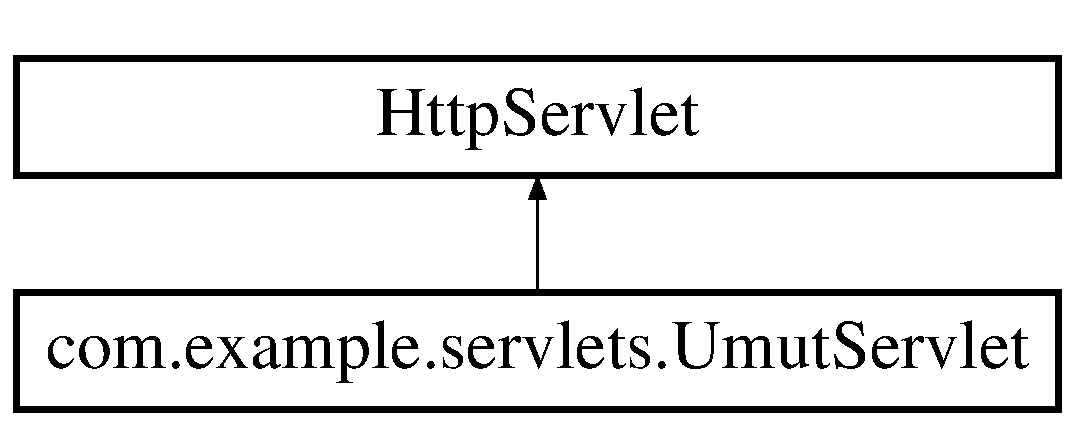
\includegraphics[height=2.000000cm]{classcom_1_1example_1_1servlets_1_1_umut_servlet}
\end{center}
\end{figure}
\subsection*{Public Member Functions}
\begin{DoxyCompactItemize}
\item 
\hyperlink{classcom_1_1example_1_1servlets_1_1_umut_servlet_a187d7bf04e87a540c3d2b52c44c14cf3}{Umut\+Servlet} ()
\end{DoxyCompactItemize}
\subsection*{Protected Member Functions}
\begin{DoxyCompactItemize}
\item 
void \hyperlink{classcom_1_1example_1_1servlets_1_1_umut_servlet_a4dba74dc02d5fe491b718022fe0e3298}{do\+Get} (Http\+Servlet\+Request request, Http\+Servlet\+Response response)  throws Servlet\+Exception, I\+O\+Exception 
\item 
void \hyperlink{classcom_1_1example_1_1servlets_1_1_umut_servlet_a10d9e55aee3af4c8023325a534f6b484}{do\+Post} (Http\+Servlet\+Request request, Http\+Servlet\+Response response)  throws Servlet\+Exception, I\+O\+Exception 
\end{DoxyCompactItemize}
\subsection*{Static Private Attributes}
\begin{DoxyCompactItemize}
\item 
static final long \hyperlink{classcom_1_1example_1_1servlets_1_1_umut_servlet_a2ac8210ed285393de2a441e311db1ea5}{serial\+Version\+U\+I\+D} = 1\+L
\end{DoxyCompactItemize}


\subsection{Detailed Description}
Written for the personal part of Assignment 6 \begin{DoxyAuthor}{Author}
dabager Umut M. Dabager \href{mailto:dabager@outlook.com}{\tt dabager@outlook.\+com} 2015700165 
\end{DoxyAuthor}
\begin{DoxyVersion}{Version}
1 
\end{DoxyVersion}


\subsection{Constructor \& Destructor Documentation}
\hypertarget{classcom_1_1example_1_1servlets_1_1_umut_servlet_a187d7bf04e87a540c3d2b52c44c14cf3}{}\index{com\+::example\+::servlets\+::\+Umut\+Servlet@{com\+::example\+::servlets\+::\+Umut\+Servlet}!Umut\+Servlet@{Umut\+Servlet}}
\index{Umut\+Servlet@{Umut\+Servlet}!com\+::example\+::servlets\+::\+Umut\+Servlet@{com\+::example\+::servlets\+::\+Umut\+Servlet}}
\subsubsection[{Umut\+Servlet()}]{\setlength{\rightskip}{0pt plus 5cm}com.\+example.\+servlets.\+Umut\+Servlet.\+Umut\+Servlet (
\begin{DoxyParamCaption}
{}
\end{DoxyParamCaption}
)}\label{classcom_1_1example_1_1servlets_1_1_umut_servlet_a187d7bf04e87a540c3d2b52c44c14cf3}
Default constructor. 

\subsection{Member Function Documentation}
\hypertarget{classcom_1_1example_1_1servlets_1_1_umut_servlet_a4dba74dc02d5fe491b718022fe0e3298}{}\index{com\+::example\+::servlets\+::\+Umut\+Servlet@{com\+::example\+::servlets\+::\+Umut\+Servlet}!do\+Get@{do\+Get}}
\index{do\+Get@{do\+Get}!com\+::example\+::servlets\+::\+Umut\+Servlet@{com\+::example\+::servlets\+::\+Umut\+Servlet}}
\subsubsection[{do\+Get(\+Http\+Servlet\+Request request, Http\+Servlet\+Response response)}]{\setlength{\rightskip}{0pt plus 5cm}void com.\+example.\+servlets.\+Umut\+Servlet.\+do\+Get (
\begin{DoxyParamCaption}
\item[{Http\+Servlet\+Request}]{request, }
\item[{Http\+Servlet\+Response}]{response}
\end{DoxyParamCaption}
) throws Servlet\+Exception, I\+O\+Exception\hspace{0.3cm}{\ttfamily [protected]}}\label{classcom_1_1example_1_1servlets_1_1_umut_servlet_a4dba74dc02d5fe491b718022fe0e3298}
\begin{DoxySeeAlso}{See also}
Http\+Servlet\+::do\+Get(\+Http\+Servlet\+Request request, Http\+Servlet\+Response response) 
\end{DoxySeeAlso}
Check for the input parameter and redirect.\hypertarget{classcom_1_1example_1_1servlets_1_1_umut_servlet_a10d9e55aee3af4c8023325a534f6b484}{}\index{com\+::example\+::servlets\+::\+Umut\+Servlet@{com\+::example\+::servlets\+::\+Umut\+Servlet}!do\+Post@{do\+Post}}
\index{do\+Post@{do\+Post}!com\+::example\+::servlets\+::\+Umut\+Servlet@{com\+::example\+::servlets\+::\+Umut\+Servlet}}
\subsubsection[{do\+Post(\+Http\+Servlet\+Request request, Http\+Servlet\+Response response)}]{\setlength{\rightskip}{0pt plus 5cm}void com.\+example.\+servlets.\+Umut\+Servlet.\+do\+Post (
\begin{DoxyParamCaption}
\item[{Http\+Servlet\+Request}]{request, }
\item[{Http\+Servlet\+Response}]{response}
\end{DoxyParamCaption}
) throws Servlet\+Exception, I\+O\+Exception\hspace{0.3cm}{\ttfamily [protected]}}\label{classcom_1_1example_1_1servlets_1_1_umut_servlet_a10d9e55aee3af4c8023325a534f6b484}
\begin{DoxySeeAlso}{See also}
Http\+Servlet\+::do\+Post(\+Http\+Servlet\+Request request, Http\+Servlet\+Response response) 
\end{DoxySeeAlso}


\subsection{Member Data Documentation}
\hypertarget{classcom_1_1example_1_1servlets_1_1_umut_servlet_a2ac8210ed285393de2a441e311db1ea5}{}\index{com\+::example\+::servlets\+::\+Umut\+Servlet@{com\+::example\+::servlets\+::\+Umut\+Servlet}!serial\+Version\+U\+I\+D@{serial\+Version\+U\+I\+D}}
\index{serial\+Version\+U\+I\+D@{serial\+Version\+U\+I\+D}!com\+::example\+::servlets\+::\+Umut\+Servlet@{com\+::example\+::servlets\+::\+Umut\+Servlet}}
\subsubsection[{serial\+Version\+U\+I\+D}]{\setlength{\rightskip}{0pt plus 5cm}final long com.\+example.\+servlets.\+Umut\+Servlet.\+serial\+Version\+U\+I\+D = 1\+L\hspace{0.3cm}{\ttfamily [static]}, {\ttfamily [private]}}\label{classcom_1_1example_1_1servlets_1_1_umut_servlet_a2ac8210ed285393de2a441e311db1ea5}


The documentation for this class was generated from the following file\+:\begin{DoxyCompactItemize}
\item 
src/com/example/servlets/\hyperlink{_umut_servlet_8java}{Umut\+Servlet.\+java}\end{DoxyCompactItemize}

\chapter{File Documentation}
\hypertarget{_atakan_servlet_8java}{}\section{src/com/example/servlets/\+Atakan\+Servlet.java File Reference}
\label{_atakan_servlet_8java}\index{src/com/example/servlets/\+Atakan\+Servlet.\+java@{src/com/example/servlets/\+Atakan\+Servlet.\+java}}
\subsection*{Classes}
\begin{DoxyCompactItemize}
\item 
class \hyperlink{classcom_1_1example_1_1servlets_1_1_atakan_servlet}{com.\+example.\+servlets.\+Atakan\+Servlet}
\item 
class \hyperlink{classcom_1_1example_1_1servlets_1_1_atakan_servlet_1_1_mathematician}{com.\+example.\+servlets.\+Atakan\+Servlet.\+Mathematician}
\end{DoxyCompactItemize}
\subsection*{Packages}
\begin{DoxyCompactItemize}
\item 
package \hyperlink{namespacecom_1_1example_1_1servlets}{com.\+example.\+servlets}
\end{DoxyCompactItemize}

\hypertarget{_bugra_servlet_8java}{}\section{src/com/example/servlets/\+Bugra\+Servlet.java File Reference}
\label{_bugra_servlet_8java}\index{src/com/example/servlets/\+Bugra\+Servlet.\+java@{src/com/example/servlets/\+Bugra\+Servlet.\+java}}
\subsection*{Classes}
\begin{DoxyCompactItemize}
\item 
class \hyperlink{classcom_1_1example_1_1servlets_1_1_bugra_servlet}{com.\+example.\+servlets.\+Bugra\+Servlet}
\end{DoxyCompactItemize}
\subsection*{Packages}
\begin{DoxyCompactItemize}
\item 
package \hyperlink{namespacecom_1_1example_1_1servlets}{com.\+example.\+servlets}
\end{DoxyCompactItemize}

\hypertarget{_burak_servlet_8java}{}\section{src/com/example/servlets/\+Burak\+Servlet.java File Reference}
\label{_burak_servlet_8java}\index{src/com/example/servlets/\+Burak\+Servlet.\+java@{src/com/example/servlets/\+Burak\+Servlet.\+java}}
\subsection*{Classes}
\begin{DoxyCompactItemize}
\item 
class \hyperlink{classcom_1_1example_1_1servlets_1_1_burak_servlet}{com.\+example.\+servlets.\+Burak\+Servlet}
\end{DoxyCompactItemize}
\subsection*{Packages}
\begin{DoxyCompactItemize}
\item 
package \hyperlink{namespacecom_1_1example_1_1servlets}{com.\+example.\+servlets}
\end{DoxyCompactItemize}

\hypertarget{_hello_servlet_8java}{}\section{src/com/example/servlets/\+Hello\+Servlet.java File Reference}
\label{_hello_servlet_8java}\index{src/com/example/servlets/\+Hello\+Servlet.\+java@{src/com/example/servlets/\+Hello\+Servlet.\+java}}
\subsection*{Classes}
\begin{DoxyCompactItemize}
\item 
class \hyperlink{classcom_1_1example_1_1servlets_1_1_hello_servlet}{com.\+example.\+servlets.\+Hello\+Servlet}
\end{DoxyCompactItemize}
\subsection*{Packages}
\begin{DoxyCompactItemize}
\item 
package \hyperlink{namespacecom_1_1example_1_1servlets}{com.\+example.\+servlets}
\end{DoxyCompactItemize}

\hypertarget{_kerim_servlet_8java}{}\section{src/com/example/servlets/\+Kerim\+Servlet.java File Reference}
\label{_kerim_servlet_8java}\index{src/com/example/servlets/\+Kerim\+Servlet.\+java@{src/com/example/servlets/\+Kerim\+Servlet.\+java}}
\subsection*{Classes}
\begin{DoxyCompactItemize}
\item 
class \hyperlink{classcom_1_1example_1_1servlets_1_1_kerim_servlet}{com.\+example.\+servlets.\+Kerim\+Servlet}
\begin{DoxyCompactList}\small\item\em This class is written for the personal assignment 6. \end{DoxyCompactList}\end{DoxyCompactItemize}
\subsection*{Packages}
\begin{DoxyCompactItemize}
\item 
package \hyperlink{namespacecom_1_1example_1_1servlets}{com.\+example.\+servlets}
\end{DoxyCompactItemize}

\hypertarget{_ozer2_servlet_8java}{}\section{src/com/example/servlets/\+Ozer2\+Servlet.java File Reference}
\label{_ozer2_servlet_8java}\index{src/com/example/servlets/\+Ozer2\+Servlet.\+java@{src/com/example/servlets/\+Ozer2\+Servlet.\+java}}
\subsection*{Classes}
\begin{DoxyCompactItemize}
\item 
class \hyperlink{classcom_1_1example_1_1servlets_1_1_ozer2_servlet}{com.\+example.\+servlets.\+Ozer2\+Servlet}
\end{DoxyCompactItemize}
\subsection*{Packages}
\begin{DoxyCompactItemize}
\item 
package \hyperlink{namespacecom_1_1example_1_1servlets}{com.\+example.\+servlets}
\end{DoxyCompactItemize}

\hypertarget{_umut_servlet_8java}{}\section{src/com/example/servlets/\+Umut\+Servlet.java File Reference}
\label{_umut_servlet_8java}\index{src/com/example/servlets/\+Umut\+Servlet.\+java@{src/com/example/servlets/\+Umut\+Servlet.\+java}}
\subsection*{Classes}
\begin{DoxyCompactItemize}
\item 
class \hyperlink{classcom_1_1example_1_1servlets_1_1_umut_servlet}{com.\+example.\+servlets.\+Umut\+Servlet}
\end{DoxyCompactItemize}
\subsection*{Packages}
\begin{DoxyCompactItemize}
\item 
package \hyperlink{namespacecom_1_1example_1_1servlets}{com.\+example.\+servlets}
\end{DoxyCompactItemize}

%--- End generated contents ---

% Index
\backmatter
\newpage
\phantomsection
\clearemptydoublepage
\addcontentsline{toc}{chapter}{Index}
\printindex

\end{document}
